\documentclass[border=10pt]{standalone}
\usepackage{tikz}
\usetikzlibrary{arrows.meta}

\begin{document}
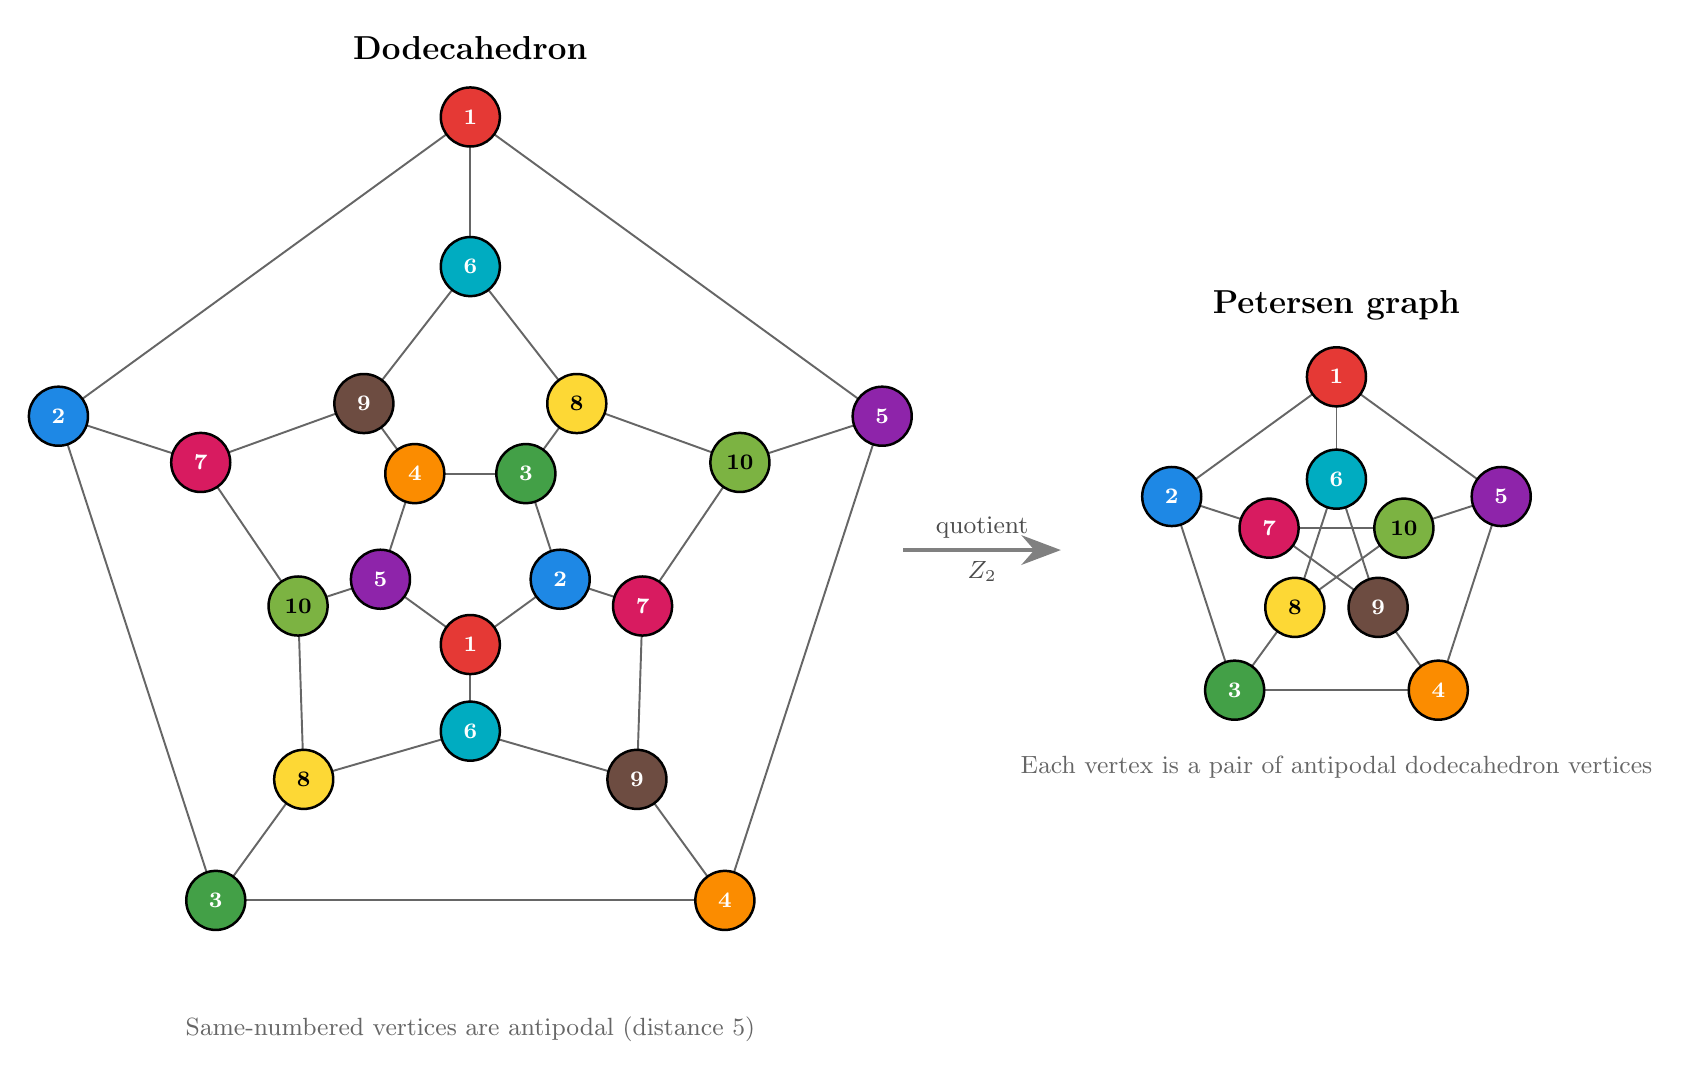
\begin{tikzpicture}[
    vtx/.style={circle, draw=black, line width=0.9pt, minimum size=7.5mm,
                inner sep=0pt, font=\footnotesize\bfseries},
    edge/.style={line width=0.7pt, black!60},
    quotarrow/.style={-{Stealth[length=5mm]}, line width=1.5pt, black!50}
]

% ============================================================
%  COLOR PALETTE (10 fibers)
% ============================================================
\definecolor{c1}{HTML}{E53935}   % red
\definecolor{c2}{HTML}{1E88E5}   % blue
\definecolor{c3}{HTML}{43A047}   % green
\definecolor{c4}{HTML}{FB8C00}   % orange
\definecolor{c5}{HTML}{8E24AA}   % purple
\definecolor{c6}{HTML}{00ACC1}   % cyan
\definecolor{c7}{HTML}{D81B60}   % pink
\definecolor{c8}{HTML}{FDD835}   % yellow
\definecolor{c9}{HTML}{6D4C41}   % brown
\definecolor{c10}{HTML}{7CB342}  % lime

% ============================================================
%  DODECAHEDRON (Schlegel diagram) — left side
% ============================================================
% Four concentric rings of 5 vertices each.
% Ring 0 (A) and Ring 1 (B): angles 90 + 72k
% Ring 2 (C) and Ring 3 (D): angles 126 + 72k  (shifted 36°)

\def\Ra{5.5}   % outer pentagon
\def\Rb{3.6}   % ring B
\def\Rc{2.3}   % ring C
\def\Rd{1.2}   % inner pentagon

% Place coordinates
\foreach \i/\ang in {1/90, 2/162, 3/234, 4/306, 5/18} {
    \coordinate (A\i) at (\ang:\Ra);
    \coordinate (B\i) at (\ang:\Rb);
}
\foreach \i/\ang in {1/126, 2/198, 3/270, 4/342, 5/54} {
    \coordinate (C\i) at (\ang:\Rc);
    \coordinate (D\i) at (\ang:\Rd);
}

% --- Edges ---
% Outer pentagon: A1-A2-A3-A4-A5-A1
\foreach \i/\j in {1/2, 2/3, 3/4, 4/5, 5/1} {
    \draw[edge] (A\i) -- (A\j);
}
% Spokes A→B
\foreach \i in {1,...,5} {
    \draw[edge] (A\i) -- (B\i);
}
% Zigzag B↔C:  B_i connects to C_i and C_{i-1}  (indices mod 5)
% B1→C1,C5  B2→C1,C2  B3→C2,C3  B4→C3,C4  B5→C4,C5
\foreach \i/\ca/\cb in {1/1/5, 2/1/2, 3/2/3, 4/3/4, 5/4/5} {
    \draw[edge] (B\i) -- (C\ca);
    \draw[edge] (B\i) -- (C\cb);
}
% Spokes C→D
\foreach \i in {1,...,5} {
    \draw[edge] (C\i) -- (D\i);
}
% Inner pentagon: D1-D2-D3-D4-D5-D1
\foreach \i/\j in {1/2, 2/3, 3/4, 4/5, 5/1} {
    \draw[edge] (D\i) -- (D\j);
}

% --- Vertices (drawn on top of edges) ---
%
% ANTIPODAL PAIRS (fibers of the covering map):
%   P1:  A1 ↔ D3      P6:  B1 ↔ C3
%   P2:  A2 ↔ D4      P7:  B2 ↔ C4
%   P3:  A3 ↔ D5      P8:  B3 ↔ C5
%   P4:  A4 ↔ D1      P9:  B4 ↔ C1
%   P5:  A5 ↔ D2      P10: B5 ↔ C2

% Outer ring A (white text on dark fill for most)
\node[vtx, fill=c1, text=white] at (A1) {1};
\node[vtx, fill=c2, text=white] at (A2) {2};
\node[vtx, fill=c3, text=white] at (A3) {3};
\node[vtx, fill=c4, text=white] at (A4) {4};
\node[vtx, fill=c5, text=white] at (A5) {5};

% Ring B
\node[vtx, fill=c6, text=white] at (B1) {6};
\node[vtx, fill=c7, text=white] at (B2) {7};
\node[vtx, fill=c8, text=black] at (B3) {8};
\node[vtx, fill=c9, text=white] at (B4) {9};
\node[vtx, fill=c10, text=black] at (B5) {10};

% Ring C  (antipodal to B, shifted by +2)
\node[vtx, fill=c9, text=white] at (C1) {9};
\node[vtx, fill=c10, text=black] at (C2) {10};
\node[vtx, fill=c6, text=white] at (C3) {6};
\node[vtx, fill=c7, text=white] at (C4) {7};
\node[vtx, fill=c8, text=black] at (C5) {8};

% Inner ring D  (antipodal to A, shifted by +2)
\node[vtx, fill=c4, text=white] at (D1) {4};
\node[vtx, fill=c5, text=white] at (D2) {5};
\node[vtx, fill=c1, text=white] at (D3) {1};
\node[vtx, fill=c2, text=white] at (D4) {2};
\node[vtx, fill=c3, text=white] at (D5) {3};

% Title
\node[font=\large\bfseries, anchor=south] at (0, \Ra+0.6) {Dodecahedron};
\node[font=\small, anchor=north, text=black!60] at (0, -\Ra-0.3)
    {Same-numbered vertices are antipodal (distance 5)};

% ============================================================
%  ARROW
% ============================================================
\draw[quotarrow] (5.5, 0) -- node[above, font=\small, text=black!70] {quotient}
                              node[below, font=\small, text=black!70] {$\mathbb{Z}_2$} (7.5, 0);

% ============================================================
%  PETERSEN GRAPH — right side
% ============================================================
\begin{scope}[xshift=11cm]

\def\Rout{2.2}
\def\Rin{0.9}

% Outer pentagon: P1–P5 at angles 90+72k
\foreach \i/\ang in {1/90, 2/162, 3/234, 4/306, 5/18} {
    \coordinate (P\i) at (\ang:\Rout);
}
% Inner pentagram: P6–P10 at angles 90+72k
\foreach \i/\ang in {6/90, 7/162, 8/234, 9/306, 10/18} {
    \coordinate (P\i) at (\ang:\Rin);
}

% Edges
% Outer cycle: 1-2-3-4-5-1
\foreach \i/\j in {1/2, 2/3, 3/4, 4/5, 5/1} {
    \draw[edge] (P\i) -- (P\j);
}
% Spokes: i to i+5
\foreach \i [evaluate=\i as \j using {int(\i+5)}] in {1,...,5} {
    \draw[edge] (P\i) -- (P\j);
}
% Inner pentagram: 6-8-10-7-9-6
\foreach \i/\j in {6/8, 8/10, 10/7, 7/9, 9/6} {
    \draw[edge] (P\i) -- (P\j);
}

% Vertices
\node[vtx, fill=c1, text=white] at (P1) {1};
\node[vtx, fill=c2, text=white] at (P2) {2};
\node[vtx, fill=c3, text=white] at (P3) {3};
\node[vtx, fill=c4, text=white] at (P4) {4};
\node[vtx, fill=c5, text=white] at (P5) {5};
\node[vtx, fill=c6, text=white] at (P6) {6};
\node[vtx, fill=c7, text=white] at (P7) {7};
\node[vtx, fill=c8, text=black] at (P8) {8};
\node[vtx, fill=c9, text=white] at (P9) {9};
\node[vtx, fill=c10, text=black] at (P10) {10};

% Title
\node[font=\large\bfseries, anchor=south] at (0, \Rout+0.6) {Petersen graph};
\node[font=\small, anchor=north, text=black!60] at (0, -\Rout-0.3)
    {Each vertex is a pair of antipodal dodecahedron vertices};

\end{scope}

\end{tikzpicture}
\end{document}
